% Gemini theme
% https://github.com/anishathalye/gemini

\documentclass[final]{beamer}

% ====================
% Packages
% ====================

\usepackage[T1]{fontenc}
\usepackage{lmodern}
\usepackage[orientation=portrait,width=36in,height=48in,scale=1.15]{beamerposter}
\usetheme{gemini}
\usecolortheme{gemini}
\usepackage{graphicx}
\usepackage[font={small}]{subcaption}
\graphicspath{{../common/personas}{../common/}{images}}
\usepackage{booktabs}
\usepackage{tikz}
\usepackage{pgfplots}
\pgfplotsset{compat=1.14}
\usepackage{anyfontsize}
\usepackage{smartdiagram}
\usesmartdiagramlibrary{additions}

% ====================
% Lengths
% ====================

% If you have N columns, choose \sepwidth and \colwidth such that
% (N+1)*\sepwidth + N*\colwidth = \paperwidth
\newlength{\sepwidth}
\newlength{\colwidth}
\newlength{\bigcolwidth}
\setlength{\sepwidth}{0.025\paperwidth}
\setlength{\colwidth}{0.45\paperwidth}
\setlength{\bigcolwidth}{0.925\paperwidth}

\newcommand{\separatorcolumn}{\begin{column}{\sepwidth}\end{column}}

% pandoc provides this command for lists
\newcommand{\pandocbounded}[1]{#1}
\providecommand{\tightlist}{%
  \setlength{\itemsep}{0pt}\setlength{\parskip}{0pt}}

% ====================
% Title
% ====================

\title{Web-connected device for personal organization}
\author{
  Mason~Becker
  \and
  Sulaiman~Islam
  \and
  Isabella~Phung
  \and
  Akanksha~Rajagopalan
  \and
  Lennan~Tuffy
}
\institute[UC Santa Cruz]{CSE 123 - Supervised by Prof. David Harrison}
\date{\today}

% ====================
% Footer (optional)
% ====================

\footercontent{
  \href{https://engineering.ucsc.edu}{https://engineering.ucsc.edu} \hfill
  Senior Design Showcase 2025, UC Santa Cruz \hfill
  % FIXME who's contact info will we use?
  \href{mailto:ltuffy@ucsc.edu}{ltuffy@ucsc.edu}}
% (can be left out to remove footer)

% ====================
% Logo (optional)
% ====================

% use this to include logos on the left and/or right side of the header:
% \logoright{\includegraphics[height=7cm]{logo1.pdf}}
\logoright{
\includegraphics[height=7cm]{BE_Logomark_CMYK_color.pdf}}
\logoleft{
\includegraphics[height=7cm]{University_of_California_Unofficial_Seal.png}}

% ====================
% Body
% ====================

\begin{document}

\begin{frame}[t]
  \begin{columns}[t]
    \separatorcolumn

    % ====================
    % Begin column 1
    % ====================
    \begin{column}{\colwidth}

      \begin{block}{Background}
        % some kind of into/hook
        % a rework of the need + goal
        The product must be a web-connected, offline capable task management
        device that keeps track of the user's habits, scheduled tasks, and 
        upcoming events.
        We created the device using the ESP-IDF platform targeting the ESP32-
        C3, with the following approach of separating the device and the 
        server:

        \begin{enumerate}
          \item \textbf{Device Implementation} Users modify the status of 
            tasks/events/habits on the device to be synced later.
          \item \textbf{Server Implementation} Users manage their data on the
            web server, producing entries that are accessible to their device.
          \item \textbf{Synchronization} Device periodically syncs by uploading
            local changes and retrieving the latest data from the server. 
        \end{enumerate}

      \end{block}

%      \begin{block}{Personas} 
%    
%    \begin{minipage}[t]{0.3\linewidth}
%      \centering
%      \includegraphics[width=0.8\linewidth]{camillia.png}
%    \end{minipage}
%    \hfill
%    \begin{minipage}[t]{0.65\linewidth}
%      \textbf{Camillia - Cardiologist}
%      
%      Cardiologist, wants to balance demanding work schedule with quality time with kids. Needs help organizing daily tasks so that she can make it to special occasions with her family.
%    \end{minipage}
%    
%    \vspace{0.5cm}
%    
%    \begin{minipage}[t]{0.3\linewidth}
%      \centering
%      
\includegraphics[width=0.8\linewidth]{Elijah.png}
%    \end{minipage}
%    \hfill
%    \begin{minipage}[t]{0.65\linewidth}
%      \textbf{Elijah - IT receptionist}
%      
%      [IT receptionist, wants to keep track of all the message assignments and dynamically edit his schedule to adapt to meeting times. Is married and wants to spend time with adopted puppy.]
%    \end{minipage}
%    
%    \vspace{0.5cm}
%    
%    \begin{minipage}[t]{0.3\linewidth}
%      \centering
%      
\includegraphics[width=0.8\linewidth]{Linda.png}
%    \end{minipage}
%    \hfill
%    \begin{minipage}[t]{0.65\linewidth}
%      \textbf{Linda - Marketing and Sales}
%      
%      [Is striving for managerial position but often struggles to find time to let loose and rest.]
%    \end{minipage}
%
%    
%    \vspace{0.4cm}
%    
%    \begin{minipage}[t]{0.3\linewidth}
%      \centering
%      
\includegraphics[width=0.8\linewidth]{Peyton.png}
%    \end{minipage}
%    \hfill
%    \begin{minipage}[t]{0.65\linewidth}
%      \textbf{Peyton - [Barista and Bartender]}
%      
%      [He works both jobs in a day and aspires to pick up new hobies and work out.]
%    \end{minipage}
%    
%    \vspace{0.4cm}
%    
%    \begin{minipage}[t]{0.3\linewidth}
%      \centering
%      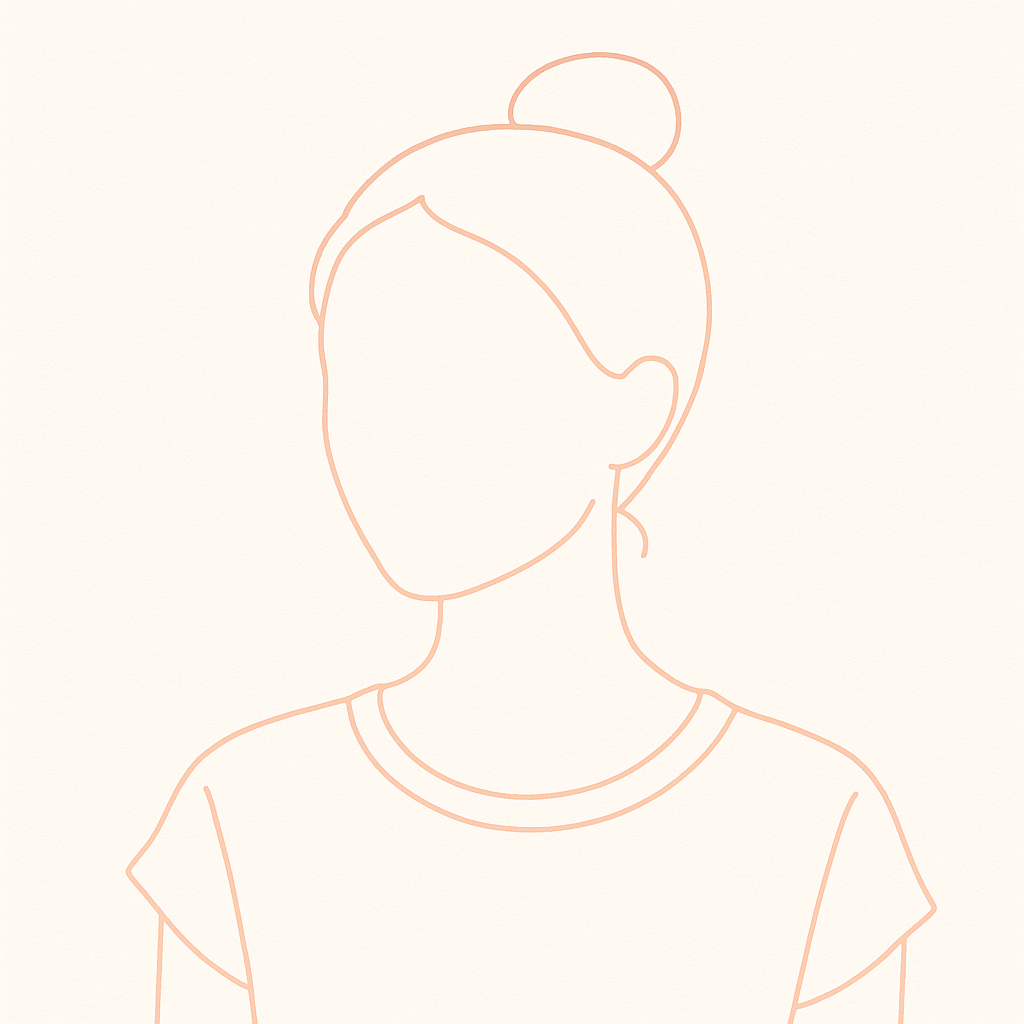
\includegraphics[width=0.8\linewidth]{Mary.png}
%    \end{minipage}
%    \hfill
%    \begin{minipage}[t]{0.65\linewidth}
%      \textbf{Mary - [University Student]}
%      
%      [She has to balance school work, chores and social life. Productivity phone apps don't help.]
%    \end{minipage}
%
%  \end{block}

      \begin{block}{System Architecture}

        \begin{figure}
          \begin{subfigure}[t]{0.54\textwidth}
              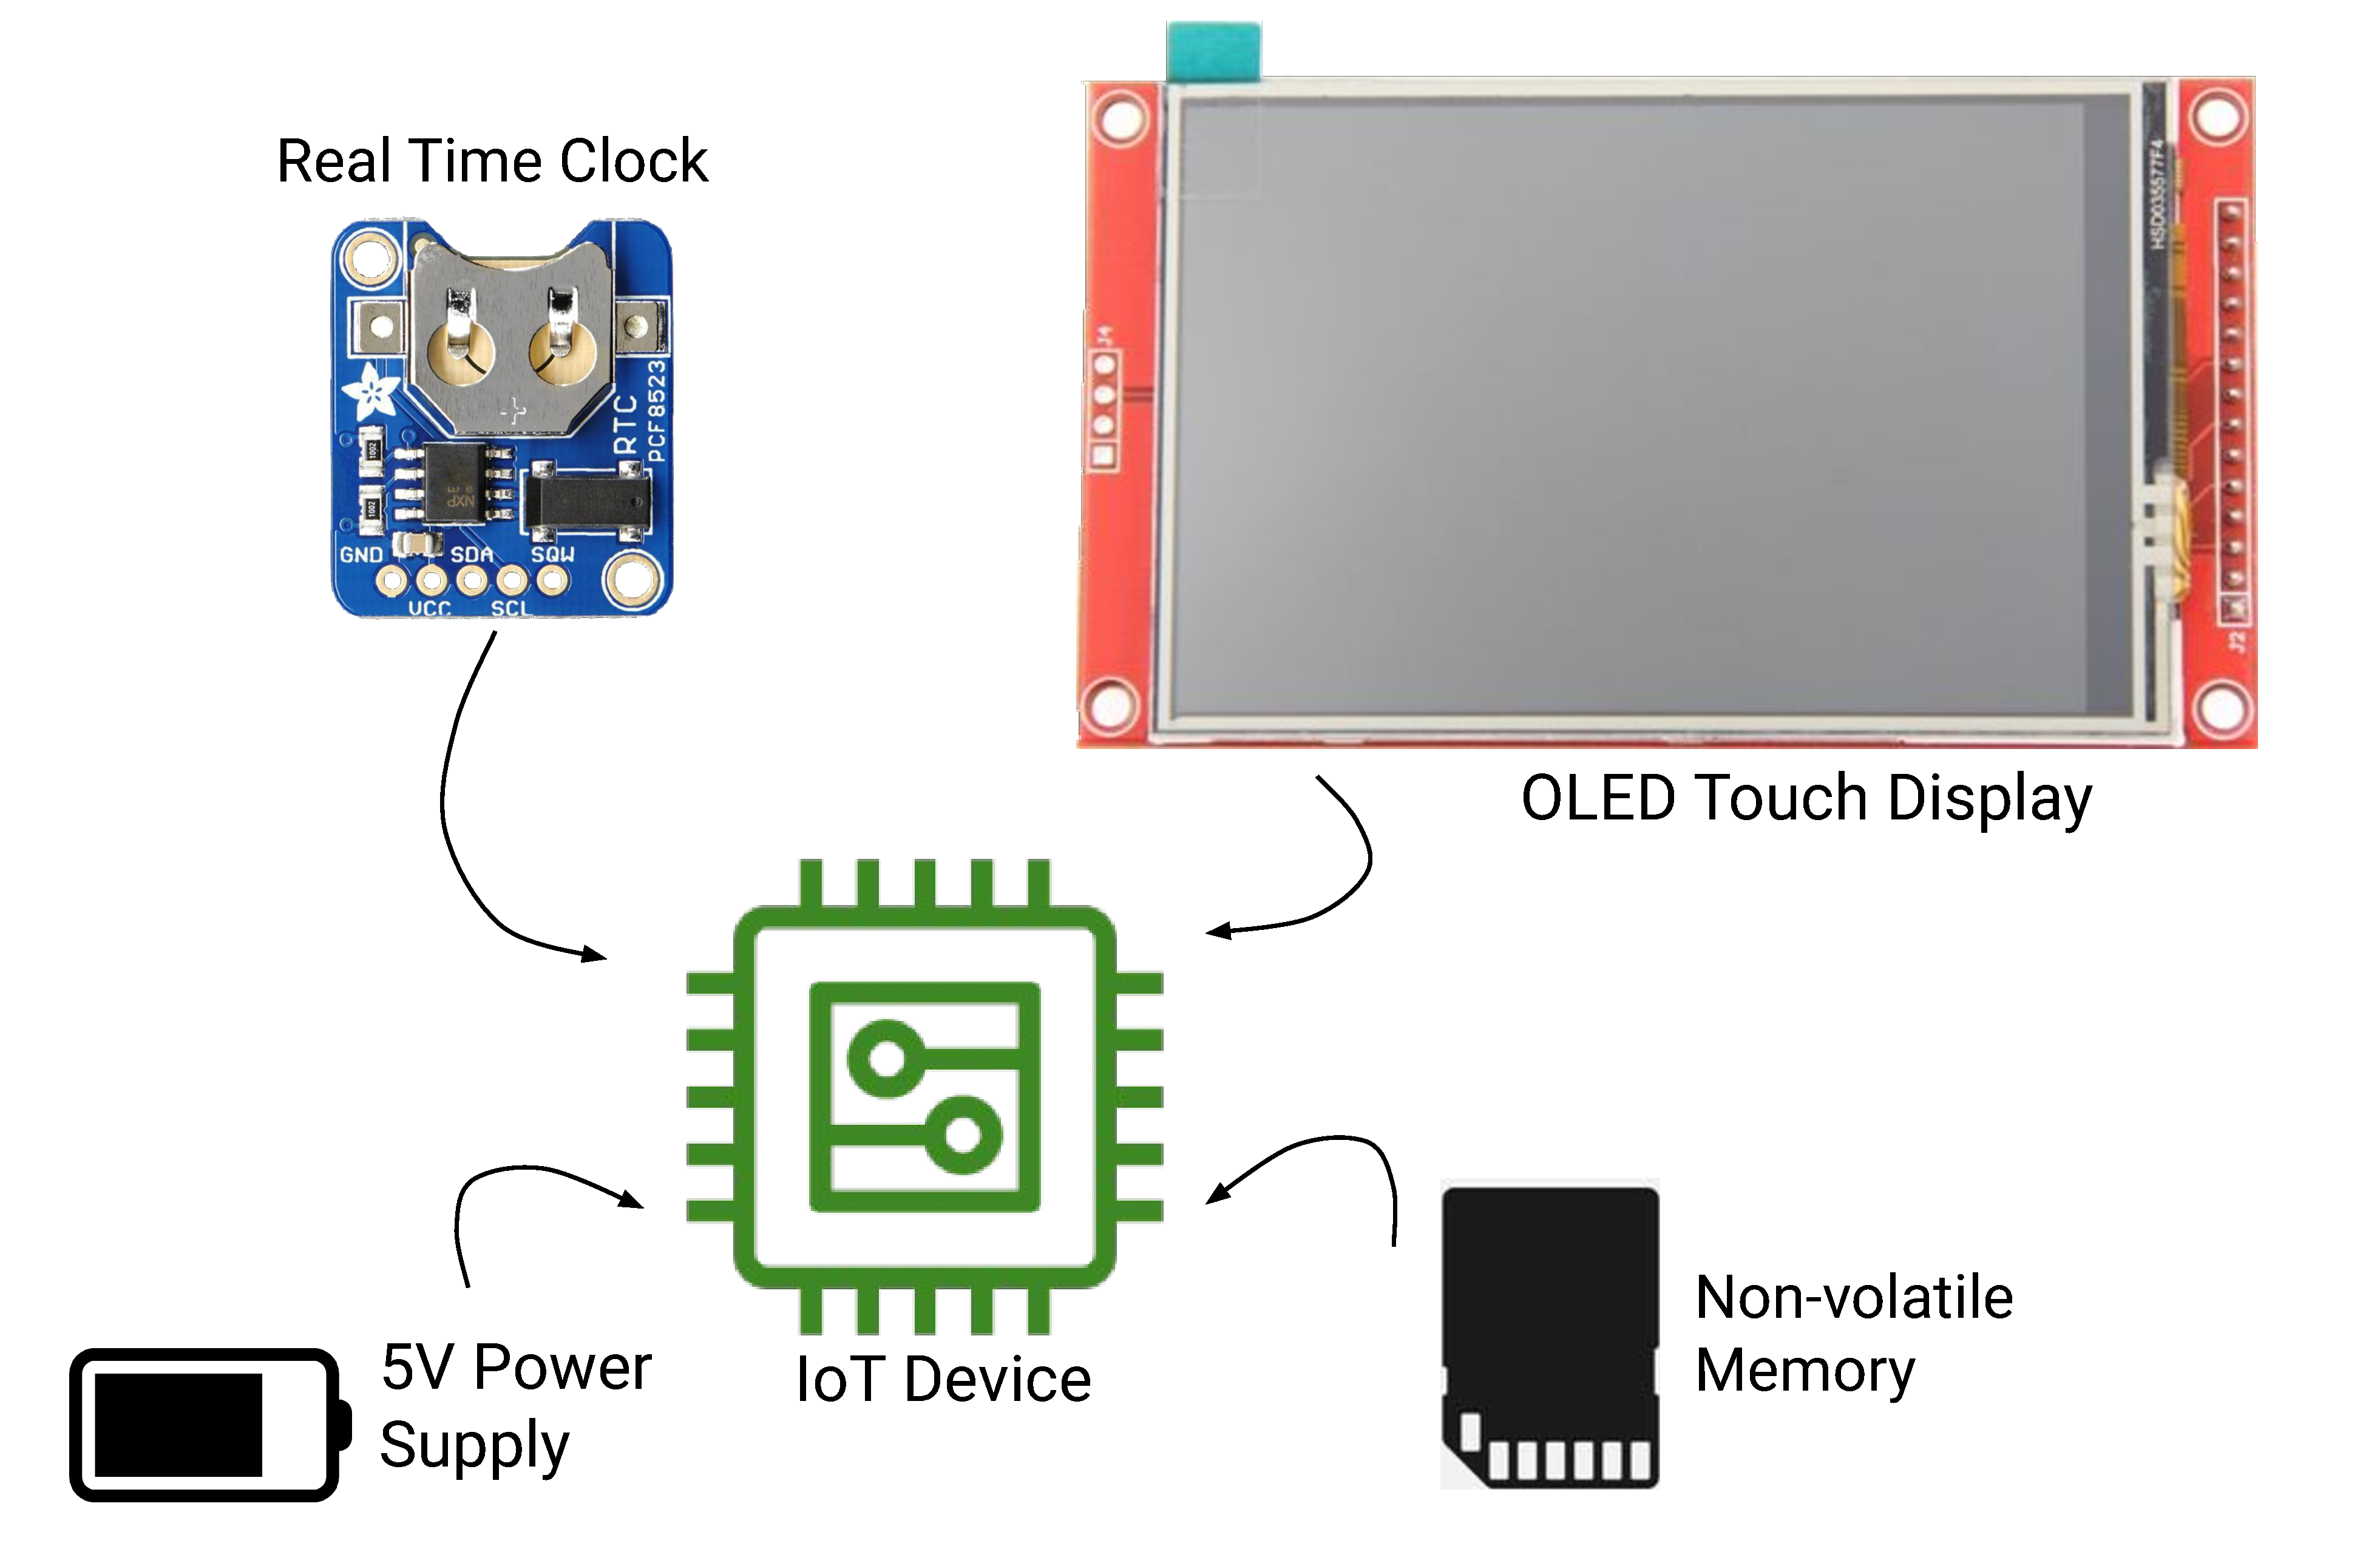
\includegraphics[width =\textwidth]{product_components.pdf}
              \caption{Component Diagram}
          \end{subfigure}
          \begin{subfigure}[t]{0.44\textwidth}
              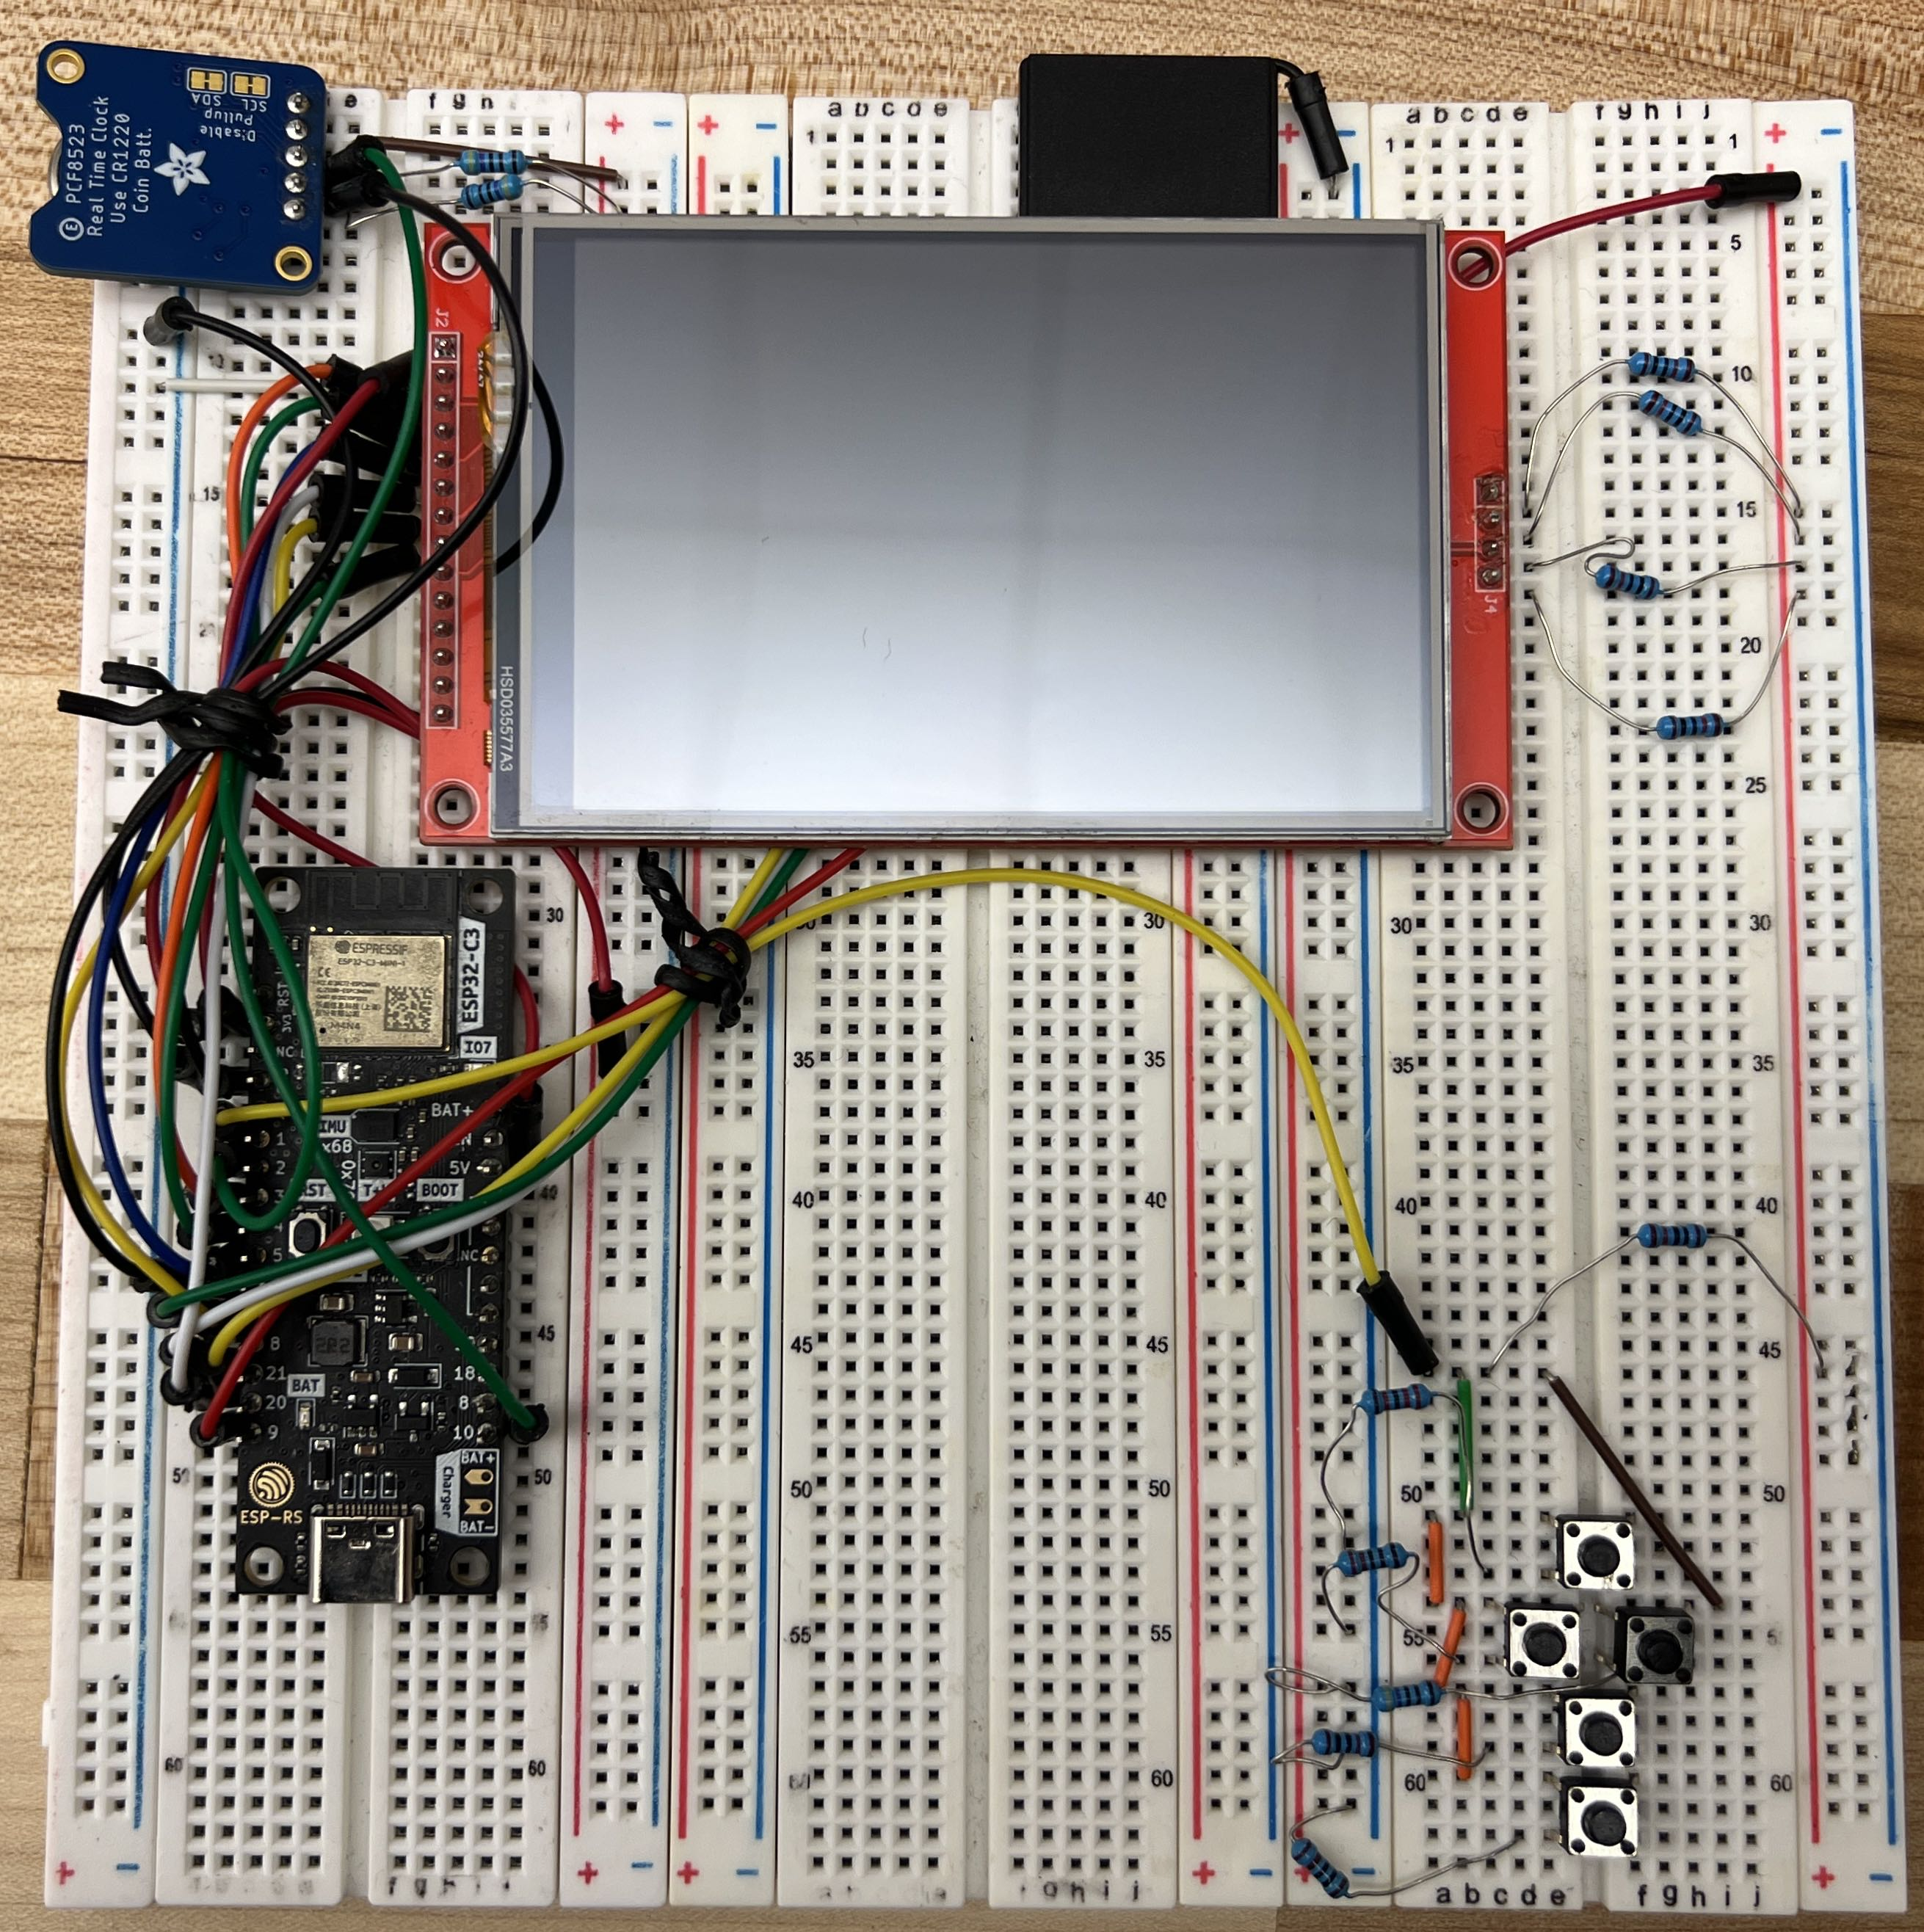
\includegraphics[width=\textwidth]{prototype.jpg}
              \caption{Functional Prototype}
          \end{subfigure}
        \end{figure}

        \begin{itemize}
          \item \textbf{Input}: Touch screen for navigating menus and
            making modifications to data.
          \item \textbf{Software}: Components manage task storage and
            management, rendering of the user interface, wireless
            communication, and initial setup.
          \item \textbf{Display}: 7.5" OLED screen displays time, connection status,
            and user data.
          \item \textbf{Persistence}: RTC maintains devices track of time even 
            when powered off, and the onboard flash memory maintains user data
            between resets.
          \item \textbf{Configuration}: Device enters access point mode during set up to allow for Wi-Fi provisioning.
        \end{itemize}

      \end{block}

     \begin{block}{User interface}

        \begin{figure}
          \centering
          \begin{subfigure}{0.49\textwidth}
            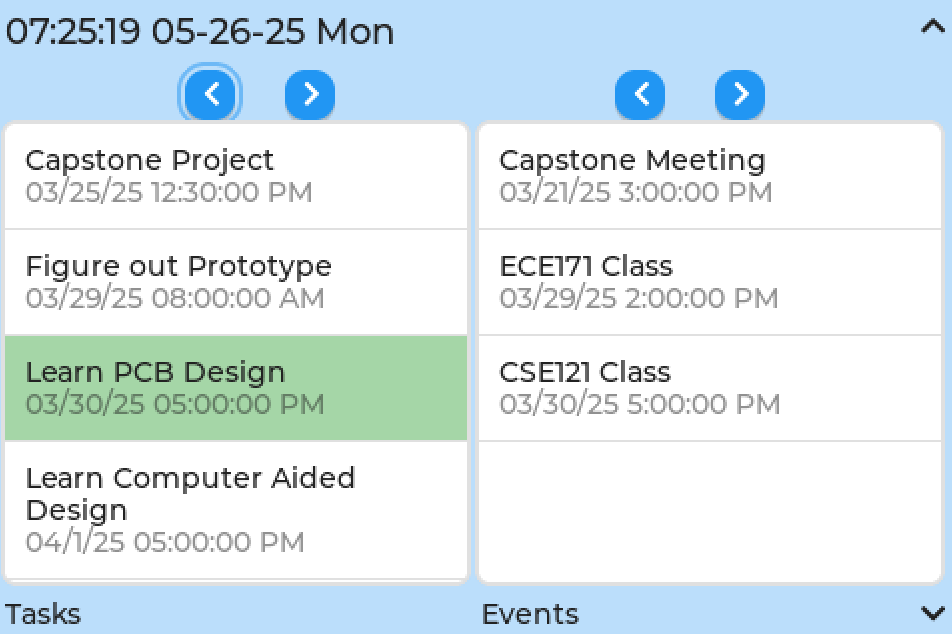
\includegraphics[width=\textwidth]{taskEvent.png}
            \caption{Main Menu}
          \end{subfigure}
          \hfill
          \begin{subfigure}{0.49\textwidth}
            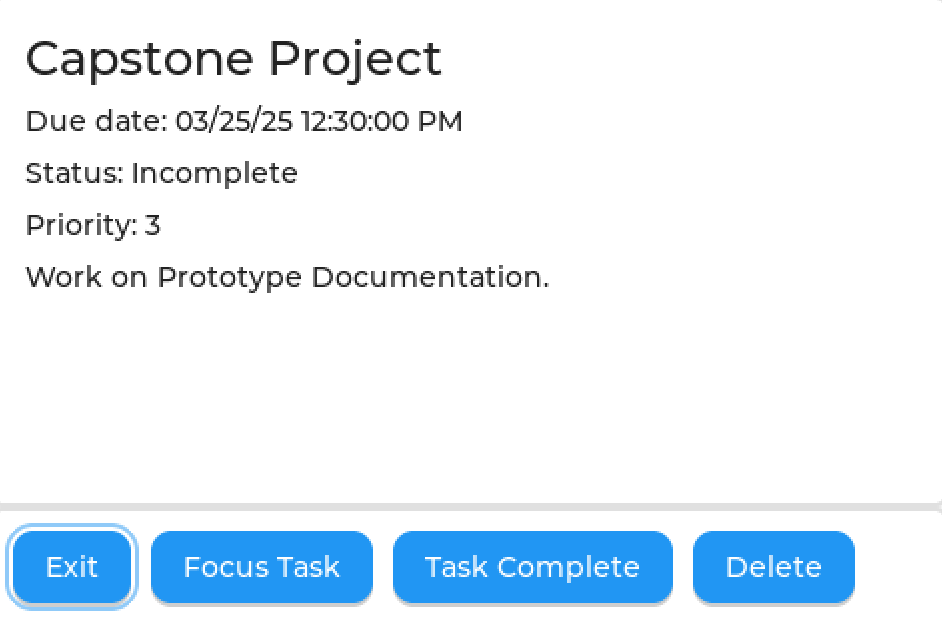
\includegraphics[width=\textwidth]{taskTile.png}
            \caption{Detailed Task View}
          \end{subfigure}
          \\
          \begin{subfigure}{0.49\textwidth}
            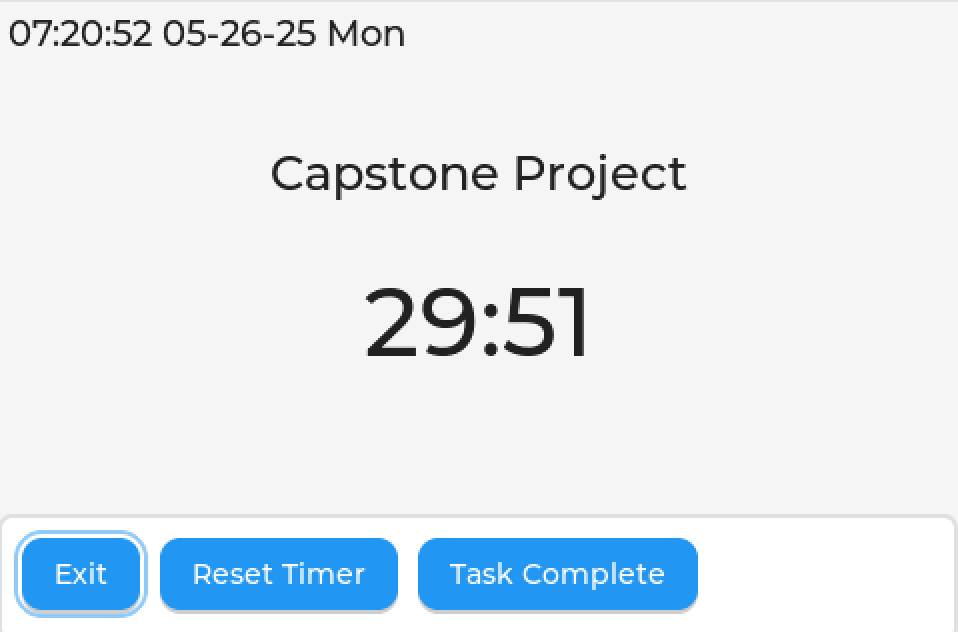
\includegraphics[width=\textwidth]{focusTile.png}
            \caption{Focus Task View}
          \end{subfigure}
          \hfill
          \begin{subfigure}{0.49\textwidth}
            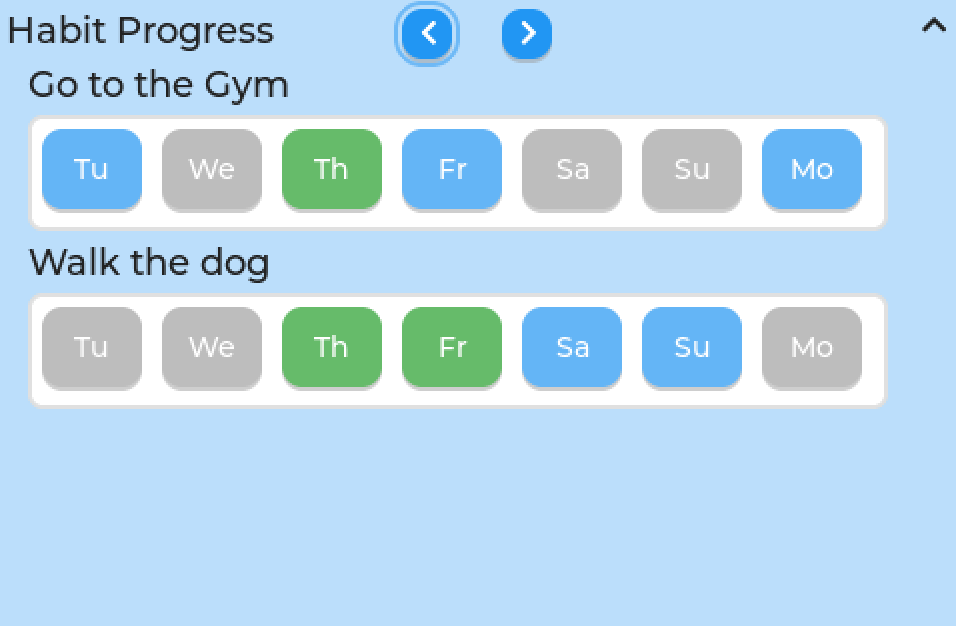
\includegraphics[width=\textwidth]{habitTile.png}
            \caption{Habit Tracking View}
          \end{subfigure}
        \end{figure} 

      \end{block}

    \end{column}
    % ====================
    % End column 1
    % ====================

    \separatorcolumn

    % ====================
    % Begin column 2
    % ====================
    \begin{column}{\colwidth} 

      \begin{block}{Goal Driven Design}

        \textbf{Entries}

        To achieve their goals and maintain a healthy routine, device includes 
        three tools to tackle the day:

        \begin{center}
          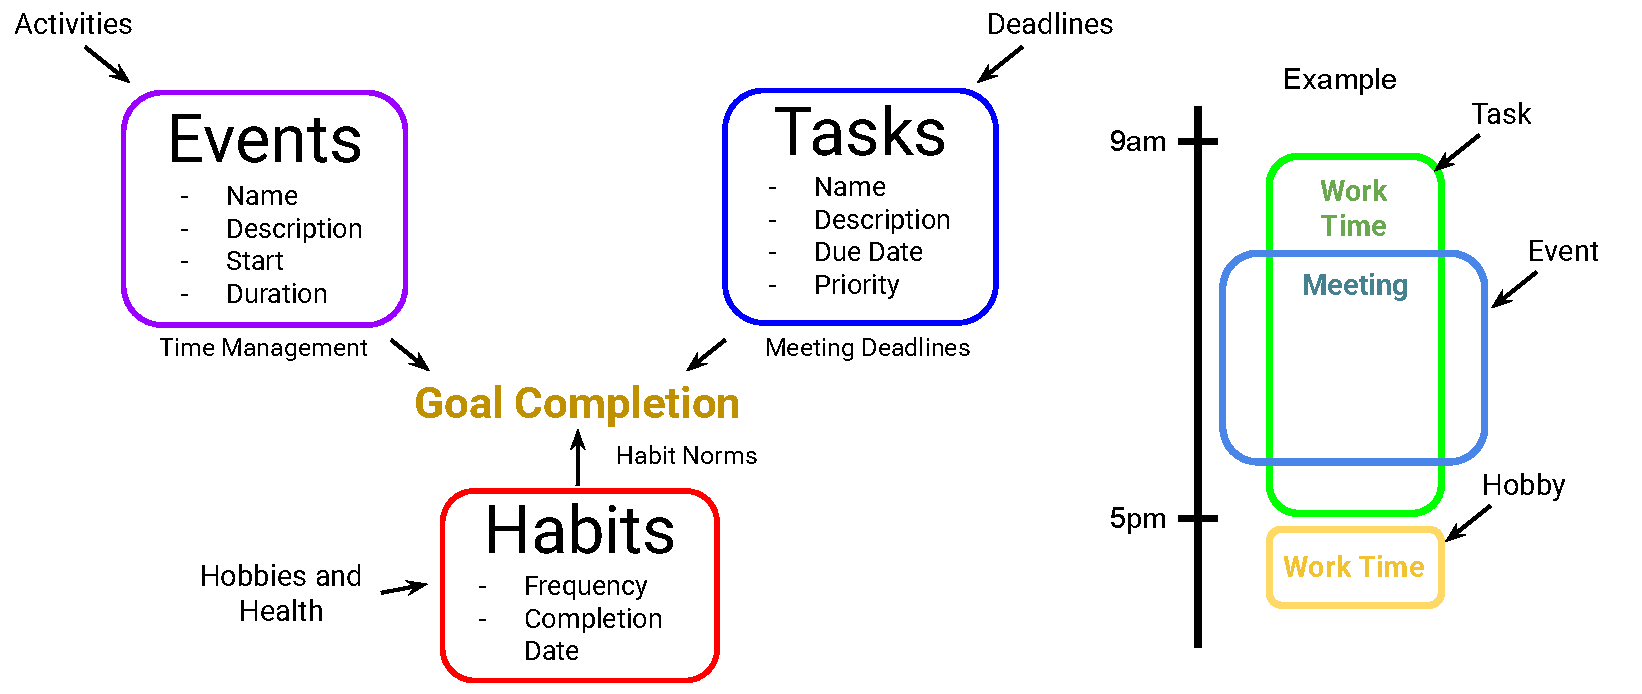
\includegraphics[width = 0.9 \textwidth]{entry_logic.pdf}
        \end{center}

      \end{block}

      \begin{block}{Web Interface}
        \begin{itemize}
          \item \textbf{Daily overview}: A landing page for a devices's data 
            that displays today's tasks, habits, and events.
          \item \textbf{Entry creation and modification}: Create and modify 
            entries to be sent to the device form the cloud.
          \item \textbf{Monthly overview}: View scheduled tasks and events in a
            calendar view.
          \item \textbf{Many-to-many usage}: multiple users may share multiple
            devices with others.
          \item \textbf{User configuration}: Sign up as a new user, or
            add/remove devices as a returning user.
        \end{itemize}
        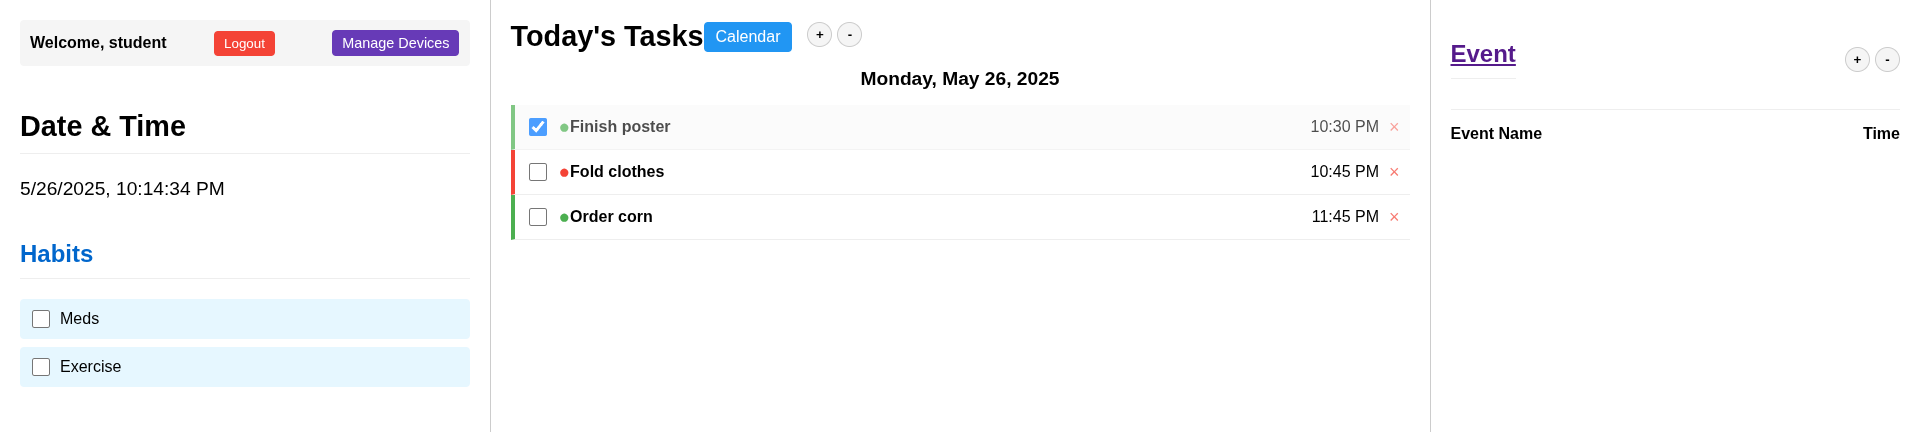
\includegraphics[width = \textwidth]{web_mainview.png}
        %\begin{figure}
        %  \begin{subfigure}{\textwidth}
        %    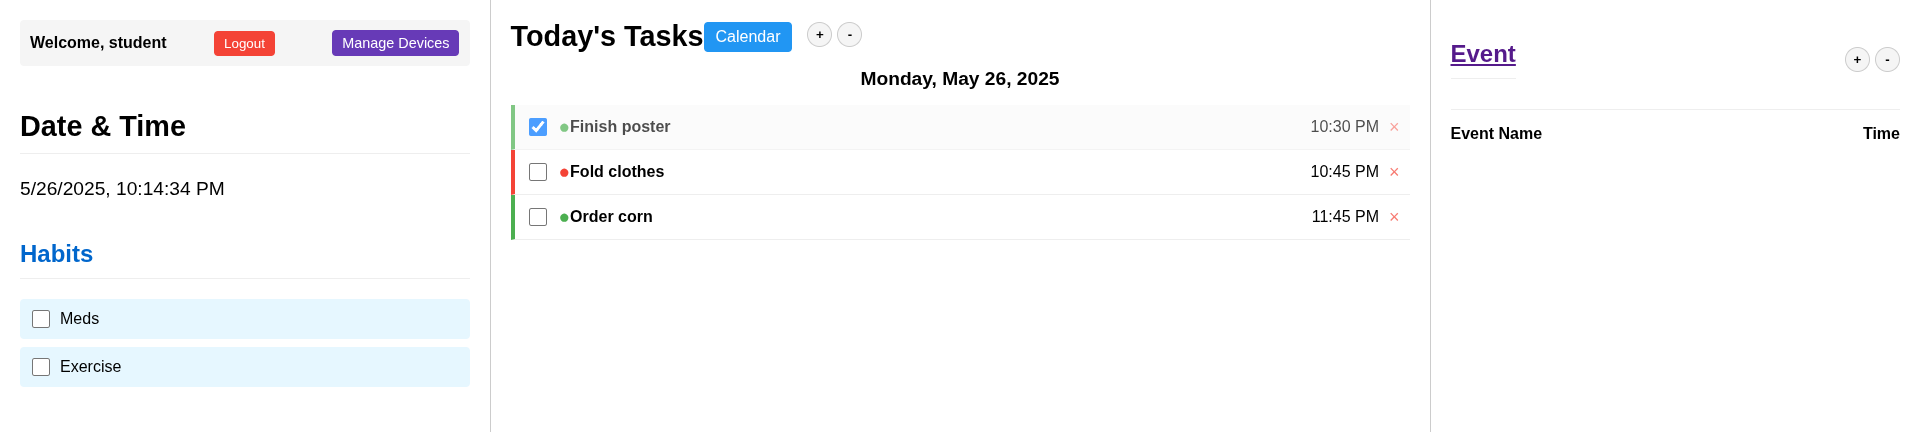
\includegraphics[width = \textwidth]{web_mainview.png}
        %    \caption{Home Page}
        %  \end{subfigure}
        %  \\
        %  \begin{subfigure}{0.49\textwidth}
        %    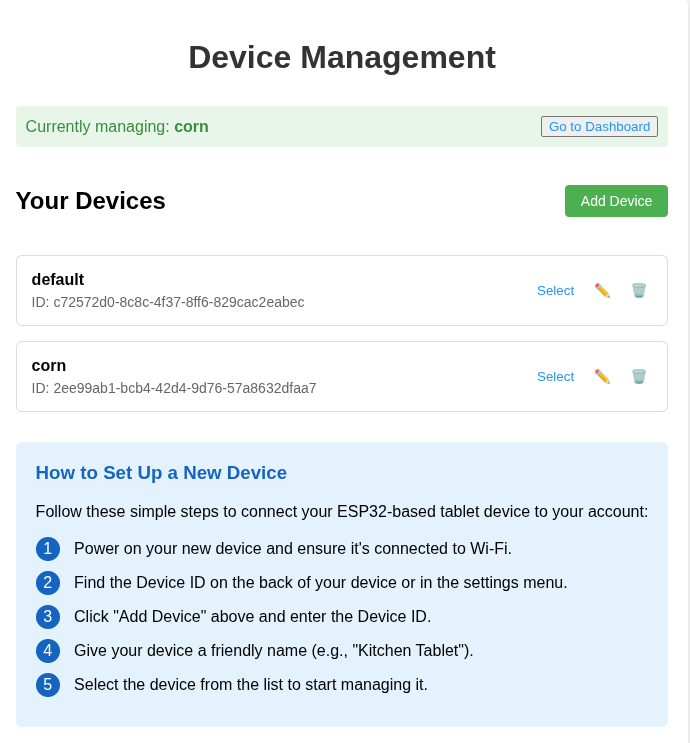
\includegraphics[width = \textwidth]{web_devices.png}
        %    \caption{Device Management}
        %  \end{subfigure}
        %  \hfill
        %  \begin{subfigure}{0.49\textwidth}
        %    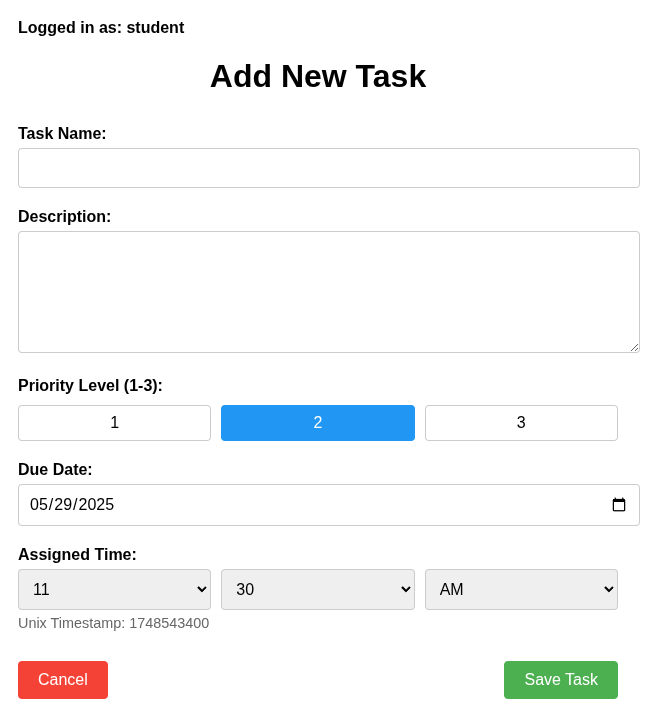
\includegraphics[width = \textwidth]{web_addtask.png}
        %    \caption{Task Creation}
        %  \end{subfigure}
        %\end{figure}
      \end{block}

      \begin{block}{Server Architecture}

        \begin{itemize}
          \item The device communicates with the cloud via MQTT
          \item Messages are routed to/from the endpoint with lambda functions
          \item The message queue and the web server both pull data from S3
          \item Server software is deployed on an EC2 
        \end{itemize}

        \vskip 0.5cm
        \begin{center}
          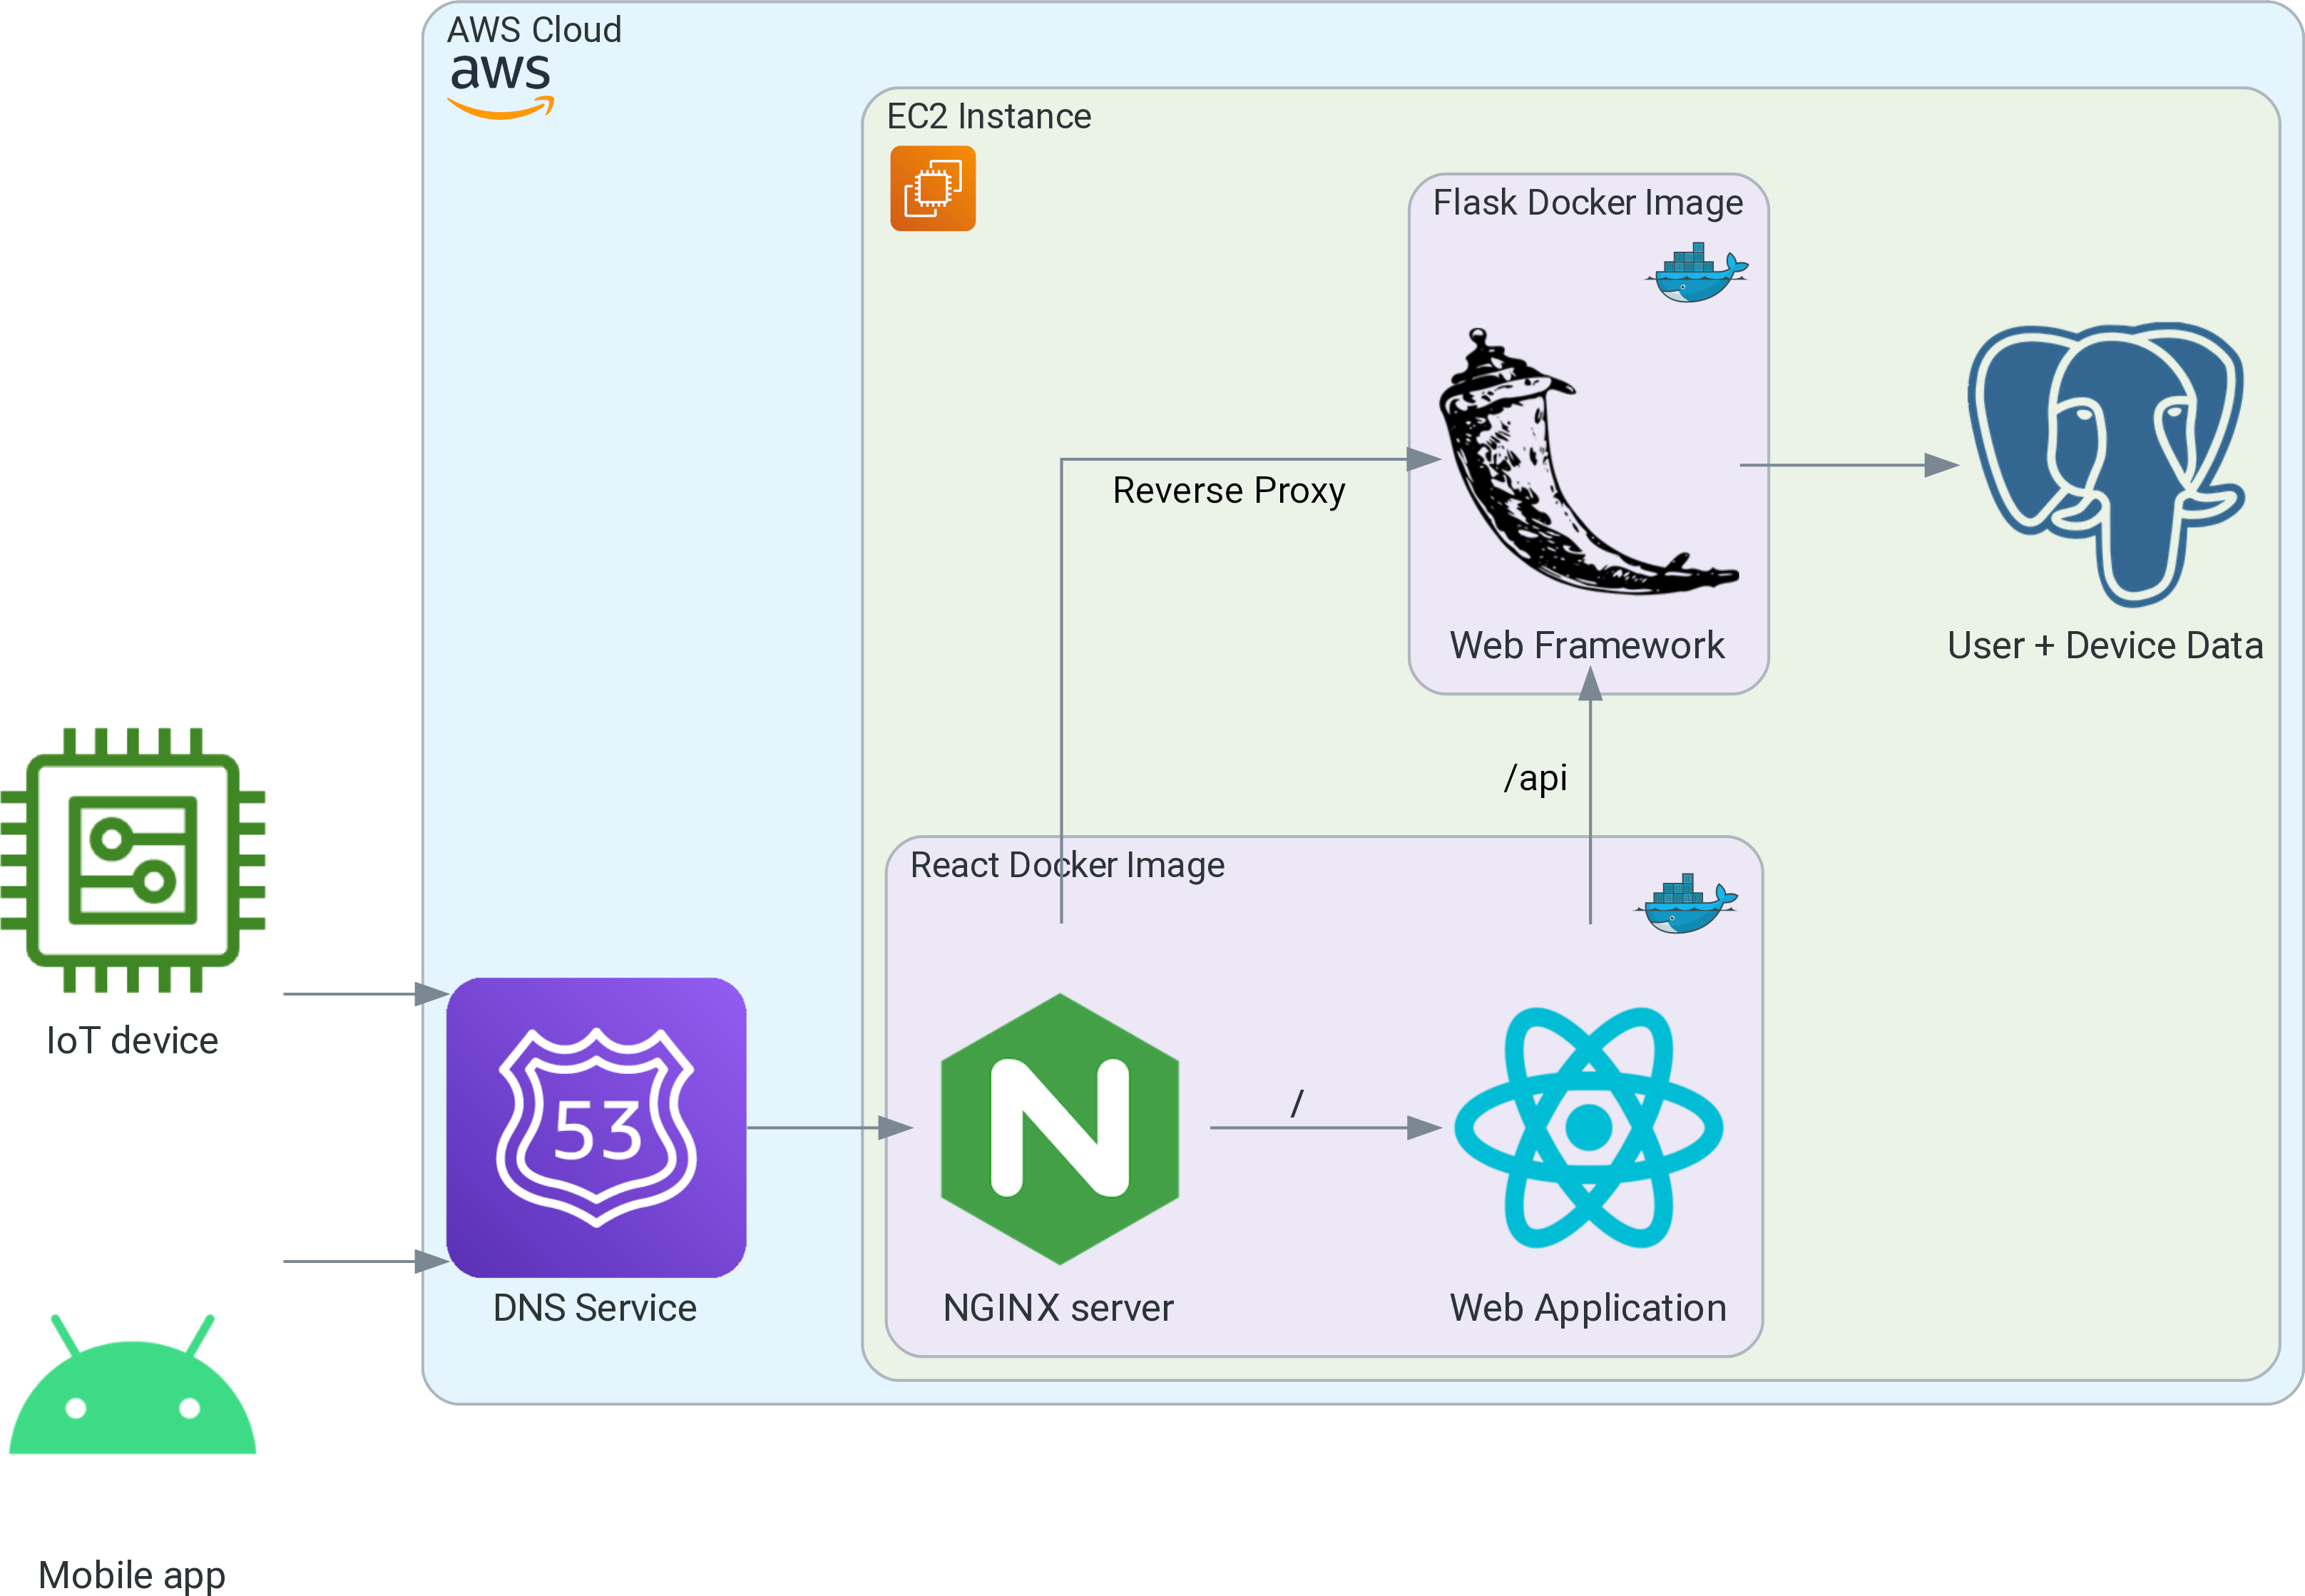
\includegraphics[width = 0.95 \textwidth]{data_flow.png}
        \end{center}
      \end{block}

    \end{column}
    % ====================
    % End column 2
    % ====================

    \separatorcolumn

  \end{columns}
\end{frame}

\end{document}
